\documentclass{beamer}

\usetheme{Szeged}
\definecolor{beamer@jana}{rgb}{0.3, 0.6, 0.8}
\setbeamercolor{structure}{fg=beamer@jana}	
\usepackage{beamerthemeshadow}
\usepackage{url}
\usepackage[utf8]{inputenc}
\usepackage{graphicx}
\usepackage{color}
\usepackage{tikz}
\usepackage{caption}
\usepackage{subcaption}
\usepackage{dirtytalk}
\usepackage{amsthm}

\usepackage[]{algorithm2e}
\usepackage{algorithmicx}
\usepackage[Algorithm,ruled]{algorithm}
\usepackage{algorithm,algcompatible,amsmath}
\usepackage{mathtools}
\algnewcommand\DESCRIPTION{\item[\textbf{Opis:}]}%
\algnewcommand\INPUT{\item[\textbf{Ulaz:}]}%
\algnewcommand\OUTPUT{\item[\textbf{Izlaz:}]}%

\usepackage{fourier} 
\usepackage{array}
\usepackage{makecell}
\renewcommand\theadalign{cc}
\renewcommand\theadfont{\bfseries}
\renewcommand\theadgape{\Gape[2pt]}
\renewcommand\cellgape{\Gape[2pt]}

\usepackage{amsmath,bm}
\usepackage{adjustbox}

\setbeamertemplate{footline}{\hspace*{.5cm}\scriptsize{\hspace*{50pt} \hfill\hspace*{.5cm}}\\
\vspace{20pt}}

\usepackage[english,serbian]{babel}


\begin{document}
\title{\Large Metode za rešavanje problema simboličke regresije \\ \vspace{5pt} \scriptsize {master rad}\\ \vspace{2pt}\small{Jana Jovičić 1097/2019}\\ \vspace{2pt}\small{mentor: dr Aleksandar Kartelj}}
\institute {\tiny{Matematički fakultet\\Univerzitet u Beogradu}}
%\author{Jana Jovičić\\ \tiny 1097/2019}
\date{\tiny 10. septembar 2022.}

\setbeamertemplate{footline}
{
  \leavevmode
  \hbox{
  \begin{beamercolorbox}[wd=.49\paperwidth,ht=2.25ex,dp=1ex,center]{author in head/foot}
    \usebeamerfont{author in head/foot}{Jana Jovičić}
  \end{beamercolorbox}
  \begin{beamercolorbox}[wd=.49\paperwidth,ht=2.25ex,dp=1ex,center]{title in head/foot}
    \usebeamerfont{title in head/foot}{Master rad}
  \end{beamercolorbox}}
}


\begingroup
\setbeamertemplate{footline}{}
\begin{frame}
    \begin{tikzpicture}
        \node[anchor=north east, inner sep=2] (image) at (0,0)
        {
\includegraphics[width=1.8cm]{images/matf-light.png}};
        \node[anchor=north west, inner sep=2] (image) at (7,0)
        {
\includegraphics[width=1.3cm]{images/matf_logo.png}};
    \end{tikzpicture}
  \vspace{-0.53cm}
  \titlepage
\end{frame}
\endgroup

\setbeamertemplate{section in toc}[sections numbered]
\setbeamertemplate{subsection in toc}{\leavevmode\leftskip=3.2em\rlap{\hskip-2em\inserttocsectionnumber.\inserttocsubsectionnumber}\inserttocsubsection\par}
\setbeamerfont{subsection in toc}{size=\footnotesize}

\begin{frame}\frametitle{Sadržaj}\tableofcontents
\end{frame} 

\section{Uvod} 
\begin{frame} {Motivacija} 
\begin{itemize}
    \item Lakša analiza različitih fizičkih sistema.
    \item Modelovanje osobina različitih fizičkih sistema pomoću promenljivih i razumevanje odnosa između tih promenljivih.
    \item Pronalazak modela kojim se najbolje opisuje dostupni skup podataka.
    \item Ne zahteva prethodnu specifikaciju strukture modela, već istovremeno uči i o strukturi modela i njegove parametre.
    \item Pod manjim uticajem ljudske greške ili nedovoljnog domenskog znanja u odnosu na regresione metode koje unapred pretpostavljaju formu modela.
    \item Prednost u odnosu na metode dubokog učenja je u lakšoj interpretabilnosti.
\end{itemize}

\end{frame}

\begin{frame}{Tip problema}
\begin{itemize}
    \item Problem kombinatorne optimizacije.
    \item Instance velikih dimenzija je nemoguće rešiti usled ograničenja vremenskih i memorijskih resursa.
    \item Najčešće se traže aproksimativna rešenja problema, uglavnom pomoću razlčitih metaheurističkih metoda.
    \item Smatra se da je NP-težak problem, ali još nije formalno dokazano.
\end{itemize}
\end{frame}

%%%%%%%%%%%%%%%%%%%%%%%%%%%%%%%%%%%%%%%%%%%%%%%%%%%%%
\section{Pojam simboličke regresije}
\subsection{Regresija}
\begin{frame}{Regresija}
\begin{itemize}
    \item Tehniku za modelovanje veze izmed̄u zavisne (ciljne) promenljive i jedne ili više nezavisnih promenljivih (atributa).
    \item Cilj - formiranje modela koji će na osnovu dostupnih uzoraka za trening i odgovarajućih izlaznih vrednosti predvidati vrednost kontinualne izlazne promenljive za novi uzorak.
    \item Različiti tipovi regresione analize: linearna regresija, polinomijalna regresija, simbolička regresija.
\end{itemize}

\end{frame}

\begin{frame}{Linearna regresija}
\begin{itemize}
    \item Pretpostavlja se linearna forma modela, tj. važi pretpostavka da se vrednost ciljne promenljive može dobiti kao linearna kombinacija vrednosti ulaznih obeležja.
    \item Kako se pretpostavlja linearnu zavisnost po parametrima $\beta_0$, $\beta_1$, ..., $\beta_m$ između atributa $x_1$, $x_2$, ..., $x_m$ i ciljne promenljive $y$, onda se $y$ predstavlja u obliku
    \[ y = \beta_0 + \beta_1 x_1 + \beta_2 x_2 + ... + \beta_m x_m .\]
\end{itemize}
\end{frame}

\begin{frame}{Polinomijalna regresija}
\begin{itemize}
    \item Veza izmed̄u atributa i ciljne promenljiv se modeluje pomoću polinoma $n$-tog stepena.
    \item U slučaju jedne nezavisne promenljive, ciljna promenljiva je oblika
    \[ y = \beta_0 + \beta_1 x_1 + \beta_2 x_1^{2} + ... + \beta_m x_1^{m} \] 
    \item Ovakav model se i dalje smatra linearnim, jer su težine pridružene atributima linearne. Samo je kriva koju modelujemo polinomijalnog obilka.
\end{itemize}

\begin{figure}[!ht]
\begin{center}
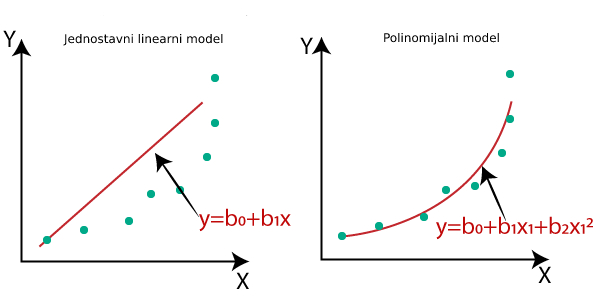
\includegraphics[width=0.55\textwidth]{images/polynomial_regression.jpg}
\end{center}
\caption{Polinomijalna regresija}
\label{fig:polyReg}
\end{figure}

\end{frame}

\begin{frame}{Simbolička regresija}
\begin{itemize}
    \item Generalizacija linearne ili polinomijalne regresije, ne pretpostavlja unapred formu modela.
    \item Cilj simboličke regresije je pronalazak matematičkog izraza u simboličkoj formi, koji dobro modeluje vezu izmed̄u ciljne promenljive i nezavisnih promenljivih.
    \item Formalno, ako je dat skup podataka $(X_i, y_i)$, $i=1,...,n$, gde $X_i \in \mathbb{R}^{n}$ predstavlja $i$-ti skup atributa, a $y_i \in \mathbb{R}$ $i$-tu ciljnu promenljivu, cilj simboličke regresije je pronalazak funkcije $f: \mathbb{R}^{n} \rightarrow \mathbb{R}$ koja najbolje odgovara skupu podataka, odnosno za koju važi $y_i \approx f(X_i), i=1,...,n$.
\end{itemize}
\end{frame}


\subsection{Evaluacija modela simboličke regresije}
\begin{frame}{Evaluacija modela simboličke regresije}
\begin{itemize}
    \item Ranije - u terminima metaheuristike kojom je problem rešavan, na primer:
    \begin{itemize}
        \item na osnovu srednje vrednosti najboljih vrednosti funkcija prilagod̄enosti dobijenih pri većem broju nezavisnih pokretanja programa.
        \item na osnovu broja uspešnih pokretanja od ukupnog broja pokretanja programa, gde se pod uspešnim pokretanjem smatralo ono u kom postoji barem jedna jedinka koja za svaku instancu iz skupa podataka daje grešku manju od nekog definisanog praga.
    \end{itemize}
    \item Poslednjih godina - poput ostalih tipova regresije: pomoću metrika kao što su MSE, RMSE i $R^2$, uz podelu skupa podataka na trening i test deo.
\end{itemize}
\end{frame}


\subsection{Evaluacija modela simboličke regresije}
\begin{frame}{Evaluacija modela simboličke regresije}
\begin{itemize}
    \item Srednje kvadratna greška (MSE, eng. \textit{Mean Squared Error})
     \[ MSE = \frac{1}{n} \sum_{i=1}^{n}(y_i - \hat{y_i})^{2}, \]
 gde je $n$ broj uzoraka, $y_i$ stvarna vrednost ciljne promenljive za $i$-ti uzorak, a $\hat{y_i}$ predviđena vrednost.
    \item Koeficijent određenosti $R^2$ (koeficijent determinacije, eng. \textit{coefficient of determination})
    \[ R^{2} = 1-\frac{MSE}{\operatorname{Var}(y)} \]
    \item Srednje kvadratna greška se izražava u terminima veličine ciljne promenljive, dok je vrednost koeficijenta određenosti normirana.
\end{itemize}
\end{frame}



\subsection{Reprezentacija izraza kod simboličke regresije}
\begin{frame}{Reprezentacija izraza kod simboličke regresije}
\begin{itemize}
    \item Izraz se može predstaviti pomoću sintaksnog stabla.
    \item Lisovi mogu da sadrže samo terminale izraza (konstante i nezavisne promenljive iz datog skupa podataka).
    \item Unutrašnjim čvorovima su predstavljeneunarne i binarne funkcije.
    \item U okviru jednog stabla ista funkcija se može pojaviti veći broj puta. Isto važi i za konstante i promenljive.
    \item Skupovi funcija i terminala su fiksirani u skladu sa trenutnim
problemom koji se rešava.
\end{itemize}
\end{frame}


\begin{frame}{Reprezentacija izraza kod simboličke regresije}

\[ \max \left\{\frac{3}{x_{3} * 2.4} ; x_{1}-x_{2}\right\} \]

\begin{figure}[!ht]
\begin{center}
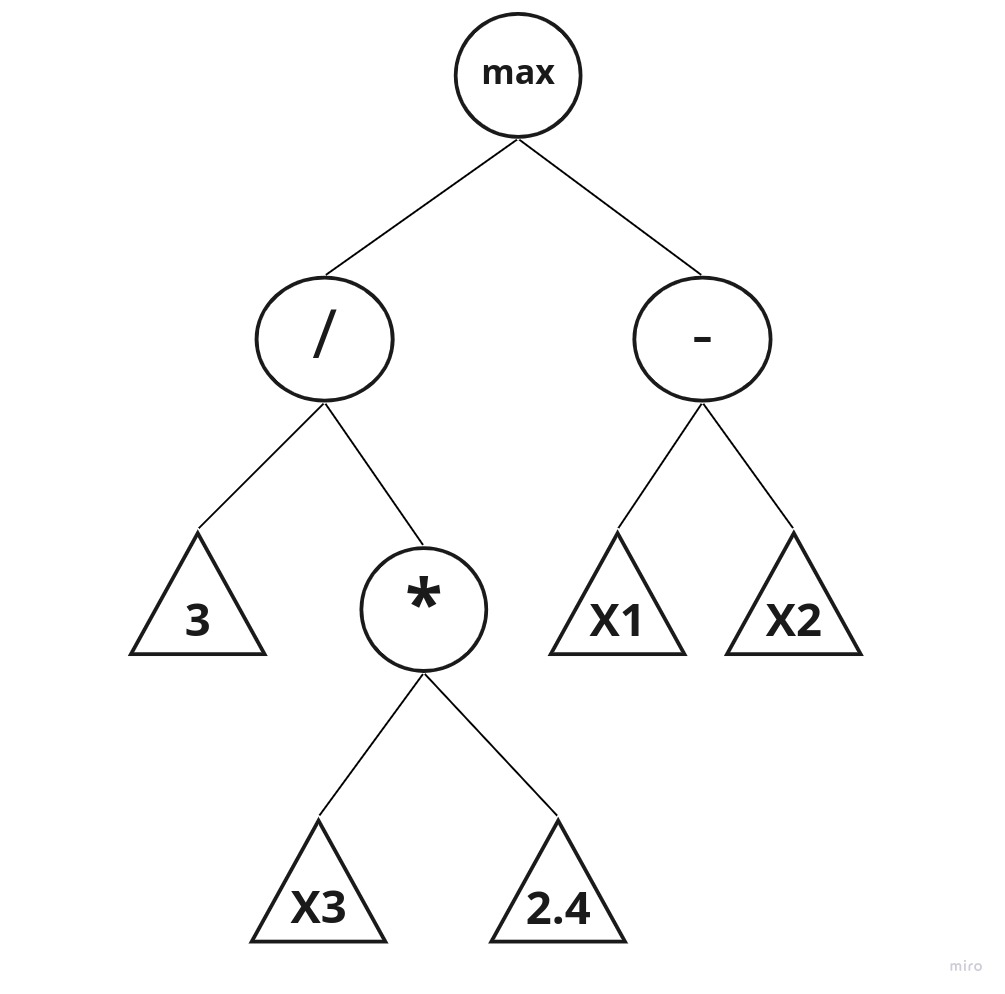
\includegraphics[width=0.4\textwidth]{images/syntax_tree.jpg}
\end{center}
\caption{Primer sintaksnog stabla}
\label{fig:syntaxTree1}
\end{figure}
\end{frame}


\begin{frame}{Reprezentacija izraza kod simboličke regresije}
\begin{itemize}
    \item Prilikom ocenjivanja tačnosti regresionog modela treba uzeti u obzir da se jedna ista funkcija može izraziti pomoću više simbolički različitih zapisa.
    \item Npr. ako je ciljna funkcija $f$ jednaka $(u + v) / (1 + uv/c^{2})$ onda se i simbolički različit zapis $(v + u) / (1 + uv/c^{2})$ treba smatrati tačnim rešenjem.
    \item Smatra se da je ciljna funkcija $f$ ispravno određena kandidatskom funkcijom $f'$ ako algebarska simplifikacija izraza $f' - f$ daje simbol "0".
\end{itemize}
\end{frame}


\section{Algoritam grube sile}
\begin{frame}{Algoritam grube sile}
\begin{itemize}
    \item Zasniva se na sistematičnoj pretrazi prostora matematičkih izraza.
    \item Pretraga podrazumeva isprobavanje svih mogućih kombinacija podizraza sve dok se ne stigne do zadovoljavajućeg rešenja.
    \item Pretraga radi iterativno po visini sintaksnog stabla izraza \cite{AIFeynman}.
    \item Prvo se proveravaju sva stabla visine 1 koja su generisana na osnovu svih datih funkcija i promenljivih. Ako među njima postoji izraz koji nad datim skupom podataka daje MSE grešku manju od definisanog parametra $\epsilon = 10^{-6}$, smatra se da je pronađeno tačno rešenje i pretraga se prekida. 
    \item Ako takav izraz nije pronađen generišu se sva stabla visine 2. Postupak se ponavlja sve dok se ne pronađe tačno rešenje ili dok se ne dostigne definisano vremensko ograničenje.
\end{itemize}
\end{frame}

\begin{frame}[fragile]{Algoritam grube sile}
\begin{figure}[!ht]
\begin{center}
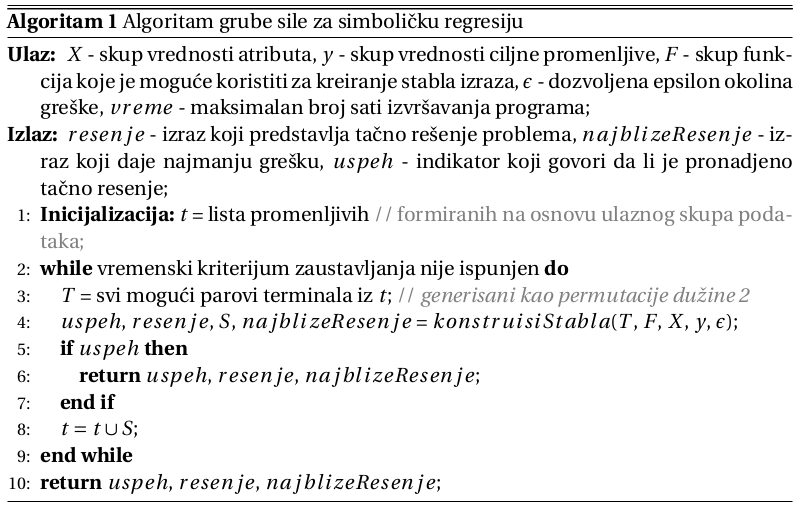
\includegraphics[width=0.80\textwidth]{images/brute_force_alg_1.png}
\end{center}
\label{fig:polyReg}
\end{figure}
\end{frame}


\begin{frame}{Algoritam grube sile}
\begin{figure}[!ht]
\begin{center}
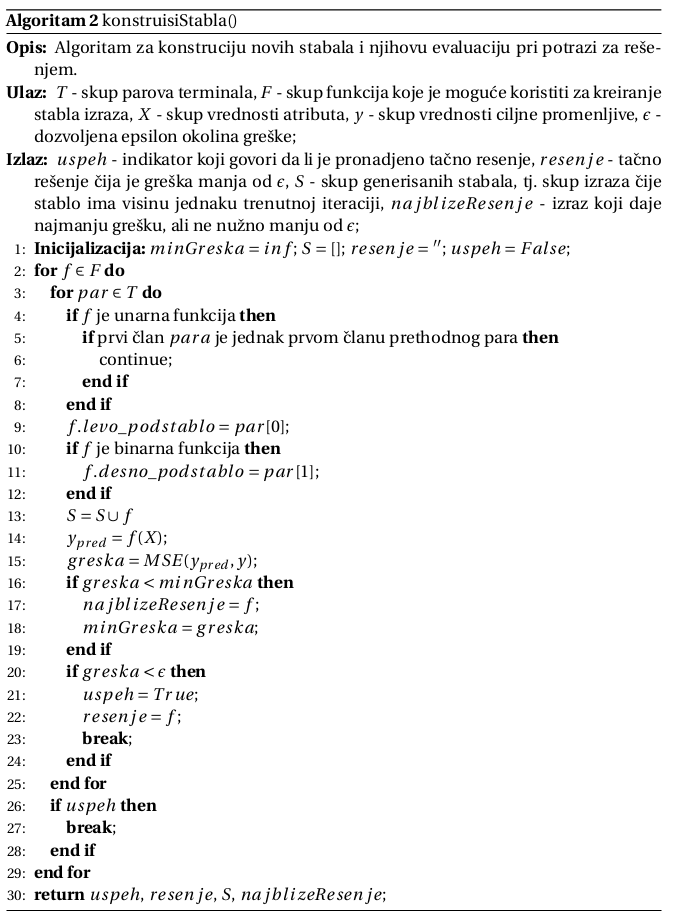
\includegraphics[width=0.45\textwidth]{images/brute_force_alg_2.png}
\end{center}
\label{fig:polyReg}
\end{figure}
\end{frame}


\begin{frame}{Algoritam grube sile}
\begin{itemize}
    \item Može se desiti da algoritam grube sile ne uspe da stigne do tačnog rešenja ne samo zbog vremenskog ograničenja, već i zbog ograničenja memorijskih resursa.
    \item U svakoj iteraciji se povećava broj stabala koje je potrebno čuvati, jer ih je u narednoj iteraciji potrebno iskoristiti kao terminale.
    \item Ako je $n$ broj funkcijskih simbola, a $m$ broj parova terminala u trenutnoj iteraciji, broj stabala generisanih u toj iteraciji biće, u najgorem slučaju, jednak $n ∗ m$.
\end{itemize}
\end{frame}


\section{Metaheurističke metode}

\subsection{Genetsko programiranje}
\begin{frame}{Genetsko programiranje}

\begin{figure}[!ht]
\begin{center}
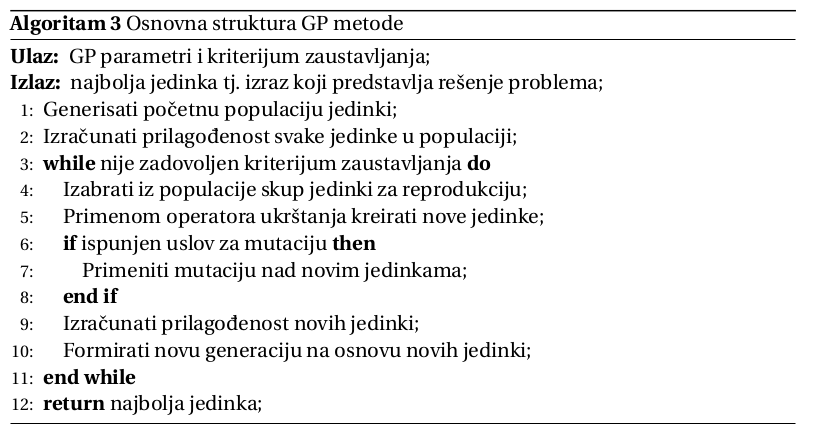
\includegraphics[width=0.75\textwidth]{images/gp_alg.png}
\end{center}
\label{fig:polyReg}
\end{figure}

\begin{itemize}
    \item Zasniva se na iterativnoj popravci inicijalne populacije rešenja.
    \item Kod GP jedinke su predstavljene stabloidinim strukturama.
    \item GP metoda je implementirana po ugledu na radove Džona Koze \cite{koza}.
\end{itemize}
\end{frame}

\begin{frame}{Reprezentacija jedinki}
\begin{itemize}
    \item Kako jedinka treba da odgovara rešenju problema, u slučaju simboličke regresije pomoću jedne jedinke je predstavljen jedan izraz koji je u obliku sintaksnog stabla.
    \item Čvorovi stabla odgovaraju unarnim i binarnim funkcijama i terminalima.
    \item Terminali mogu biti:
    \begin{itemize}
        \item promenljive definisane na osnovu dostupnog skupa podataka
        \item efemerne slučajne konstante (tj.slučajno generisani brojevi određenog tipa iz definisanog intervala, najčešće realni brojevi iz intervala [-1, 1])
    \end{itemize}
\end{itemize}
\end{frame}

\begin{frame}{Generisanje početne populacije}
\begin{enumerate}
    \item "full" metoda
        \begin{itemize}
            \small 
            \item Generisanje potpunog stabla.
            \item Put između korena i svakog lista je jednak definisanoj maksimalnoj dubini.
            \item Ako se trenutni čvor koji se generiše nalazi na dubini koja je manja od maksimalne, može se izabrati samo čvor koji predstavlja funkciju.
            \item Ako se trenutni čvor koji se generiše nalazi na dubini koja je jednaka maksimalnoj, onda se može odabrati samo terminal.
            \item Ako je trenutni čvor koji se generiše na dubini koja je manja od minimalne, moguće je odabrati samo funkciju.
        \end{itemize}
    
\end{enumerate}
\end{frame}


\begin{frame}{Generisanje početne populacije}
\begin{enumerate}
\setcounter{enumi}{1}
    \item "grow" metoda
        \begin{itemize}
            \item Generisanje stabala čiji oblici variraju.
            \item Dužina puta od korena do bilo kog lista ne bude veća od definisane maksimalne dubine, a dozvoljeno je da bude kraća.
            \item Ako se trenutni čvor koji se generiše nalazi na dubini koja je manja od maksimalne, može se izabrati ili čvor koji predstavlja funkciju ili čvor koji predstavlja terminal.
            \item Ako se trenutni čvor koji se generiše nalazi na dubini koja je jednaka maksimalnoj, onda se može odabrati samo terminal. 
            \item Ako je trenutni čvor koji se generiše na dubini koja je manja od minimalne, moguće je odabrati samo funkciju.
        \end{itemize}
\end{enumerate}
\end{frame}

\begin{frame}{Generisanje početne populacije}
\begin{enumerate}
\setcounter{enumi}{2}
    \item "ramped half-and-half" metoda
        \begin{itemize}
            \item Generisanje stabala različitih visina i oblika.
            \item Kombinacija "full" i "grow" metoda.
            \item Kreiranje podjednakog broja stabala po svakom nivou dubine od nivoa 2 do nivoa definisanog parametrom maksimalne dubine.
            \item Npr. ako je definisana maksimalna dubina jednaka 6, onda će 20\% stabala imati dubinu 2, ..., 20\% dubinu 6.
            \item Za svaki nivo dubine 50\% stabala se kreira pomoću "full", a 50\% pomoću "grow" metode.
        \end{itemize}
\end{enumerate}
\end{frame}

\begin{frame}{Funkcija prilagođenosti}
\begin{itemize}
    \item Daje ocenu kvaliteta jedinke i utiče na verovatnoću izbora te jedinke za proces formiranja nove generacije.
    \item Koza definiše 4 vrste funkcija prilagod̄enosti:
    \begin{enumerate}
    \item "Raw" funkcija prilagođenosti
    \item Standardizovana funkcija prilagođenosti 
    \item "Adjusted" funkcija prilagođenosti 
    \item Normalizovana funkcija prilagođenosti
    \end{enumerate}
\end{itemize}
\end{frame}

\begin{frame}{"Raw" funkcija prilagođenosti}
\begin{itemize}
    \item Izražava se u terminima problema koji se rešava.
    \item Kod simboličke regresije se može posmatrati kao funkcija greške.
    \item Njena vrednost za neku jedinku odgovara zbiru distanci između vrednosti koje daje izraz predstavljen tom jedinkom i pravih ciljnih vrednosti svih uzoraka iz trening skupa.
    \item  Distanca se računa kao apsolutna vrednost razlike između predviđenih i pravih vrednosti.
    \[ r(i,t) = \sum_{i=1}^{N}|y_i - \hat{y_i}|  \]
    \item Bolje jedinke imaju manju vrednost funkcije.
\end{itemize}
\end{frame}

\begin{frame}{Standardizovana funkcija prilagođenosti}
\begin{itemize}
    \small
    \item Redefiniše "raw" funkciju tako da njena vrednost za bolje jedinke uvek bude manja, bez obzira na vrstu problema koji se rešava.
    \item Kako je kod simboličke regresije "raw" funkcija već definisana tako da manje vrednosti reprezentuju bolje jedinke, standardizovana funkcija će biti jednaka "raw" funkciji.
    \[ s(i,t) = r(i,t) \]
    \item Kod problema kod kojih je "raw" prilagođenost definisana tako da se boljim jedinkama smatraju one sa većom vrednošću te funkcije, standardizovana funkcija bi bila jednaka razlici maksimalne moguće vrednosti "raw" funkcije  i vrednosti "raw" funkcije za datu jedinku.
    \[ s(i,t) = r_{max} - r(i,t). \]
\end{itemize}
\end{frame}

\begin{frame}{"Adjusted" funkcija prilagođenosti}
\begin{itemize}
    \small
    \item Računa se na osnovu standardizovane funkcije.
    \[ a(i,t) = \frac{1}{1 + s(i,t)}. \]
    \item Vrednost $a(i,t)$ pripada intervalu [0,1] i veća je za bolje jedinke.
    \item Prednost: naglašava razliku između dobrih i vrlo dobrih jedinki.
    \item Npr. ako imamo dve loše jedinke čije su vrednosti standardizovane funkcije redom 64 i 65, njihove vrednosti prilagođene funkcije će biti 0.0154 i 0.0156. U oba slučaja, razlika između prilagođenosti ove dve loše jedinke nije velika. 
    \item Ako imamo dve dobre jedinke čije su vrednosti standardizovane funkcije redom 4 i 3, njihove vrednosti prilagođene funkcije će biti 0.20 i 0.25. Ovde, iako su jedinke na osnovu vrednosti standardizovane funkcije bliske, na osnovu "adjusted" funkcije se dodatno ističe bolja od dve posmatrane dobre jedinke.
\end{itemize}
\end{frame}

\begin{frame}{Normalizovana funkcija prilagođenosti}
\begin{itemize}
    \small
    \item Računa se na osnovu "adjusted" funkcije kao
    \[ n(i,t) = \frac{a(i,t)}{\sum_{k=1}^{M}a(k,t)}, \]
    gde je M veličina populacije.
    \item Za jedniku $i$ "adjusted" funkcija prilagođenosti se normalizuje u skladu sa "adjusted" funkcijama ostalih jedinki iz populacije.
    \item Njena vrednost pripada intervalu [0, 1].
    \item Veća je za bolje jedinke u populaciji.
    \item Zbir normalizovanih vrednosti prilagođenosti svih jedinki je jednak 1.
    \item Mana: Ako u populaciji postoji neka jedinka čiji izraz nije definisan nad svim tačkama iz skupa podataka, to će onemogućiti izračunavanje normalizovane funkcije prilagođenosti čak i jedinke koja je definisana u svim tačkama.
\end{itemize}
\end{frame}

\begin{frame}{Selekcija}
\begin{itemize}
    \item Obezbeđuje čuvanje i prenošenje dobrih osobina populacije na sledeću generaciju.
    \item Turnirska selekcija - Iz tekuće populacije se na slučajan način bira $k$ jedinki, gde $k$ predstavlja veličinu turnira, a zatim se od njih bira najbolje prilagođena jedinka.
\end{itemize}
\end{frame}


\begin{frame}{Operatori ukrštanja - Standardni operator ukrštanja}

\begin{figure}[!ht]
\begin{center}
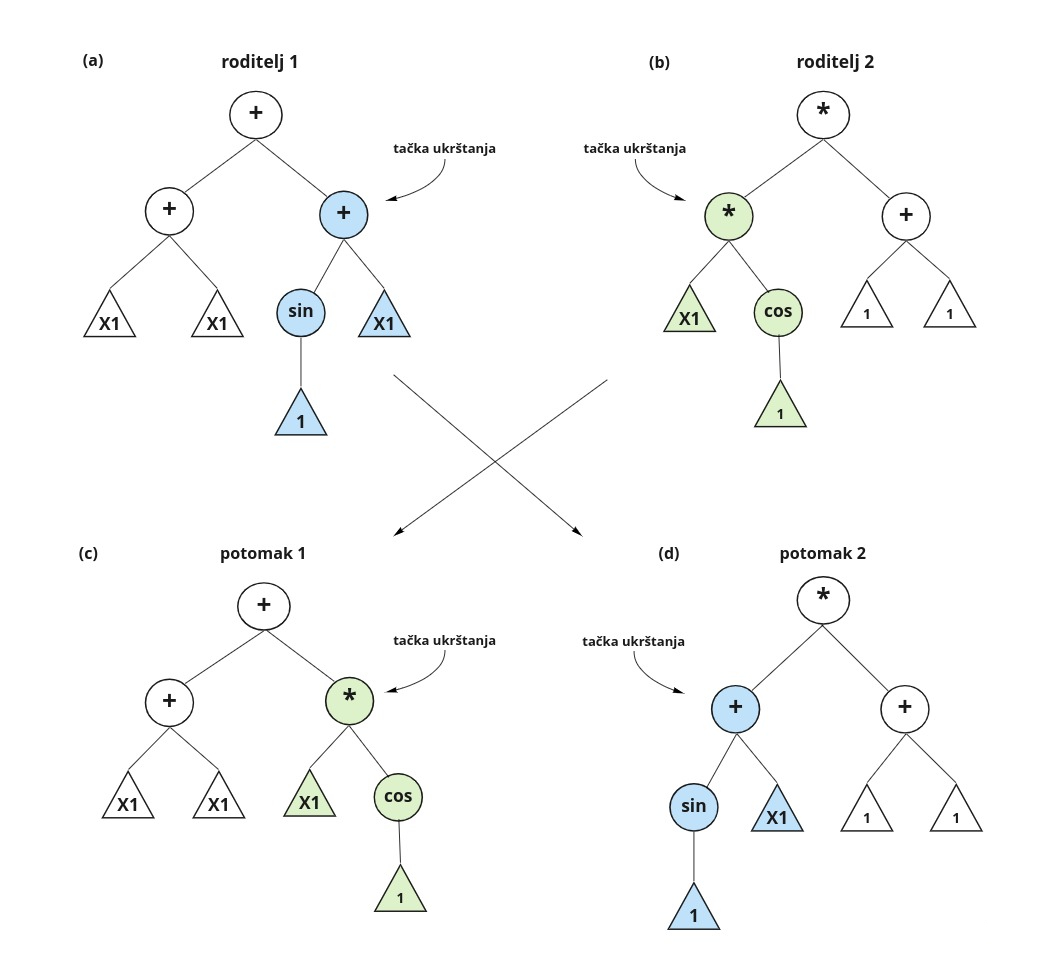
\includegraphics[width=0.65\textwidth]{images/standard_crossover4.jpg}
\end{center}
\label{fig:standardCrossover}
\end{figure}

\end{frame}


\begin{frame}{Operatori ukrštanja - Standardni operator ukrštanja}
\begin{itemize}
    \item Ukrštanje dve jedinke podrazumeva razmenu njihovih slučajno odabranih podstabala.
    \item Kod oba roditelja se odabere po jedan čvor, a zatim se razmene podstabla određena tim čvorom kao korenom.
    \item Postoji parametar kojim se ograničava veličina jedinki koje nastaju ukrštanjem.
    \item Ako se formira jedinka nedozvoljene veličine, umesto nje će u narednu generaciju ići jedan od roditelja.
\end{itemize} \end{frame}




\begin{frame}{Operatori ukrštanja - Operatori zasnovani na semantici \cite{semanticCrossover}}
\begin{itemize}
\small
    \item \textit{Semantika uzorkovanja} (SS, eng. \textit{Sampling Semantics}) nekog podstabla se aproksimira pomoću vrednosti dobijenih evaluacijom tog podstabla na predefinisanom skupu tačaka iz domena problema.
    \item Neka je $F$ funkcija koja je izražena pomoću (pod)stabla $T$ na domenu $D$ i neka je $P$ skup tačaka iz domena $D$, $P = \{p_1, p_2, ..., p_N\}$. Tada je \textit{semantika uzorkovanja} stabla $T$ na skupu $P$ u domenu $D$, skup $S = \{s_1, s_2, ..., s_N\}$ takav da je $s_i = F(p_i), i=1,2,..,N$.
    \item Na osnovu SS definiše se \textit{rastojanje semantike uzorkovanja} (SSD, \textit{Sampling Semantics Distance}) između dva podstabla. Neka je $P = \{p_1, p_2, ..., p_N\}$ \textit{semantika uzorkovanja} podstabla $St_1$, a $Q = \{q_1, q_2, ..., q_N\}$ \textit{semantika uzorkovanja} podstabla $St_2$. Onda se $SSD$ između $St_1$ i $St_2$ definiše kao 
    \[ SSD(St_1, St_2) = \frac{1}{N}(|p_1 - q_1| + |p_2 - q_2| + ... + |p_N - q_N|). \]
\end{itemize}
\end{frame}


\begin{frame}{Operatori ukrštanja - Operatori zasnovani na semantici}
\begin{itemize}
    \item Pomoću $SSD$ se definišu \textit{semantička ekvivalentnost} i \textit{semantička sličnost} između dva podstabla.
    \item Dva podstabla su \textit{semantički ekvivalentna} (SE, eng. \textit{Semantically Equivalent}) na domenu ako je njihova $SSD$ vrednost dovoljno mala
    
    \[
        SE(St_1, St_2)= 
    \begin{dcases}
        true,& \text{ako je } SSD(St_1, St_2) < \epsilon\\
        false,              & \text{inače}
    \end{dcases}
    \]
    
    \item Parametar $\epsilon$ predstavlja \textit{semantičku osetljivost} (eng. \textit{semantic sensitivity}). Za njega je najbolje uzeti neku vrednost iz skupa \{0.01, 0.02, 0.04, 0.05, 0.06, 0.08, 0.1\}.

\end{itemize}
\end{frame}
    

\begin{frame}{Operatori ukrštanja - Operatori zasnovani na semantici}
\begin{itemize}
\small
    \item Dva podstabla su \textit{semantički slična} ($SS_i$, eng. \textit{Semantically Similar}) na domenu ako njihova $SSD$ vrednost leži na nekom pozitivnom intervalu.
    \[
        SS_i(St_1, St_2)= 
    \begin{dcases}
        true,& \text{ako je } \alpha < SSD(St_1, St_2) < \beta\\
        false,              & \text{inače}
    \end{dcases}
    \]
    \item Paraametri $\alpha$ i $\beta$ donja i gornja granica semantičke osetljivosti (LBSS, eng. \textit{Lower Bound Semantic Sensitivity} i UBSS, eng. \textit{Upper Bound Semantic Sensitivity}). Kod simboličke regresije najbolje rezultate daju vrednosti između 0.4 i 0.6 za $UBSS$, a vrednosti $10^{-2}$ ili manje za $LBSS$.
    \item Motivacija za korišćenje semantičke sličnosti - verovatnije je da će razmena podstabala biti korisnija ukoliko se odvija izmed̄u dve jedinke koje nisu semantički identične, ali nisu ni semantički suviše različite.
\end{itemize}
\end{frame}

\begin{frame}{Operatori ukrštanja - Operatori zasnovani na semantici}
\small
\textbf{Operator ukrštanja koji je svestan semantike, SAC (eng. Semantics Aware Crossover)}
\begin{itemize}
    \item Onemogućavanje razmene semantički ekvivalentnih podstabala koji dovode do kreiranja potomaka koji su identični svojim roditeljima.
    
    \begin{figure}[!ht]
    \begin{center}
    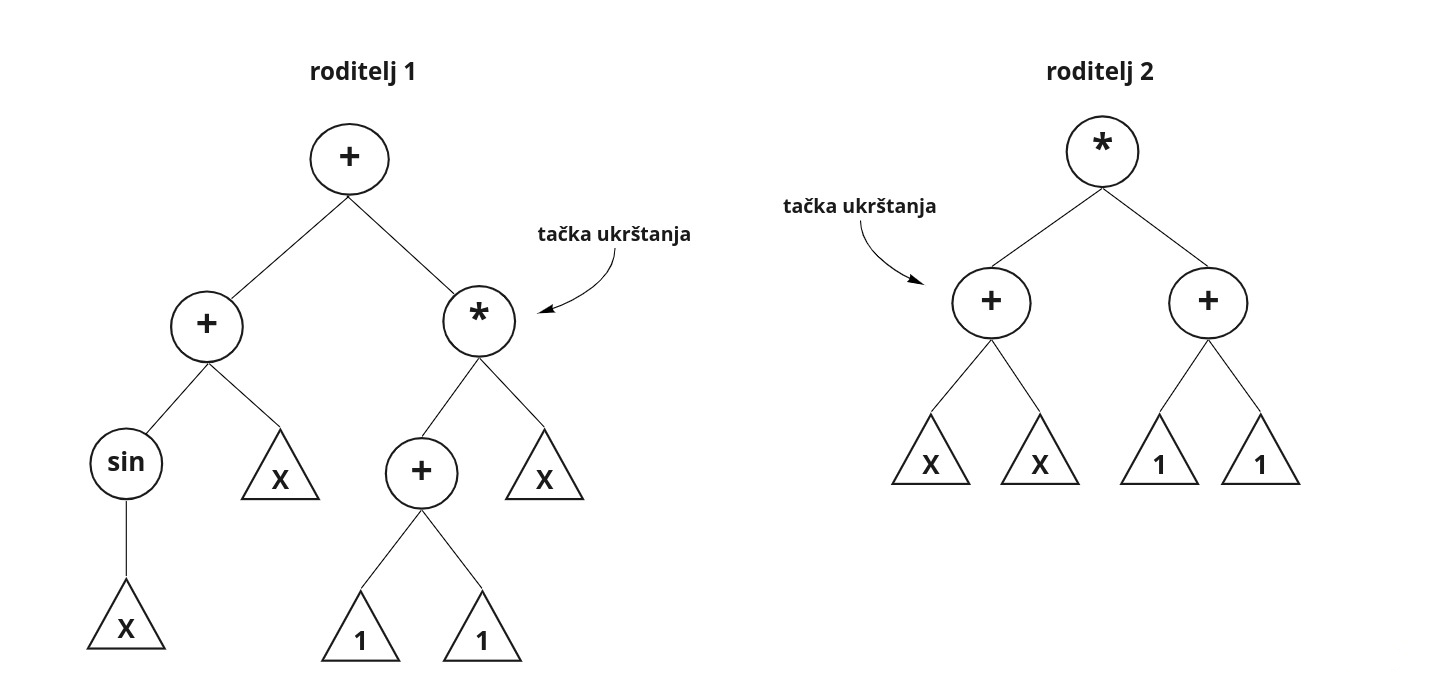
\includegraphics[width=0.6\textwidth]{images/SAC1.jpg}
    \end{center}
    \label{fig:sac1}
    \end{figure} 
    
    \item Ako su podstabla ekvivalentna, ponovo se na slučajan način biraju tačke ukrštanja.
\end{itemize}
\end{frame}


\begin{frame}{Operatori ukrštanja - Operatori zasnovani na semantici}
\small
\textbf{Operator ukrštanja koji je zasnovan na semantičkoj sličnosti, SSC (eng. Semantic Similarity-based Crossover)}
\begin{itemize}
    \item Proširenje SAC operatora.
    \item Proverava se semantička sličnost podstabala odabranih za ukrštanje.
    \item Semantičku sličnost mnogo teže zadovoljiti u odnosu na semantičku ne-ekvivalentnost, pa je verovatnije da će dolaziti do uzastopnih neuspešnih pokušaja tokom potrage za takvim podstablima.
    \item Koristi se veći broj pokušaja za pronalazak semantički sličnog para.
    \item Ako se pređe dozvoljeni broj pokušaja, podstabla se biraju na slučajan način.
\end{itemize}
\end{frame}


\begin{frame}{Operatori ukrštanja - Operatori zasnovani na semantici}
\begin{figure}[!ht]
\begin{center}
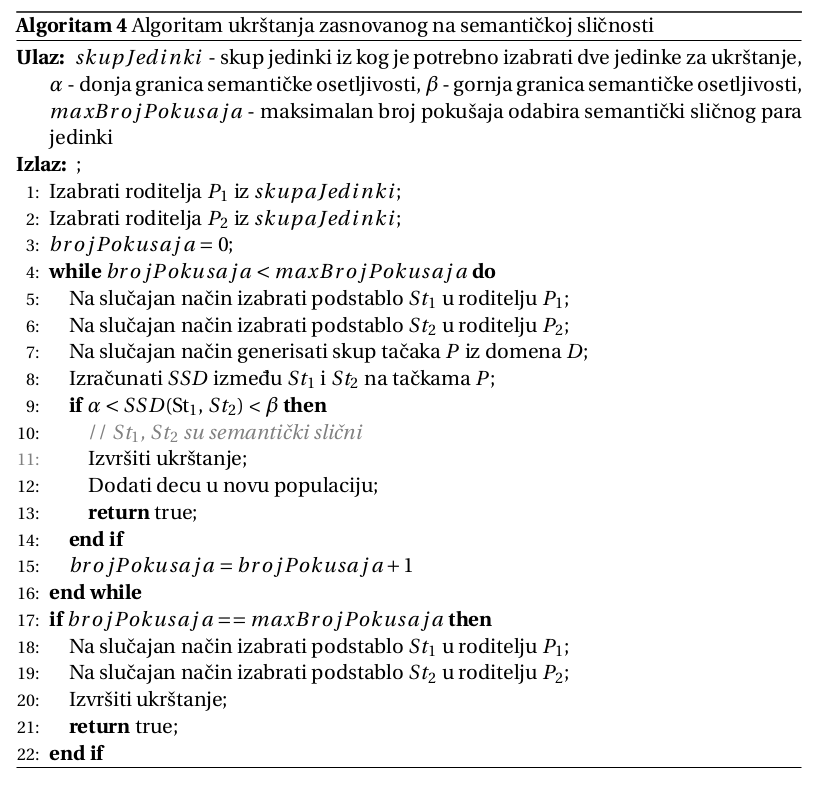
\includegraphics[width=0.6\textwidth]{images/ssc_alg.png}
\end{center}
\label{fig:sac1}
\end{figure} 
\end{frame}

\begin{frame}{Operatori mutacije}
\begin{enumerate}
    \item Mutacija pojedinačnog čvora (eng. \textit{point mutation})
    \begin{itemize}
        \item Zamena odabranog čvora nekim drugim čvorom.
        \item Terminal može biti zamenjen drugim slučajno izabranim terminalom.
        \item Funkcija može biti zamenjena drugom funkcijom iste arnosti.
    \end{itemize}
    
    \item Mutacija celog podstabla (eng. \textit{subtree mutation})
    \begin{itemize}
        \item Vrši se slučajni izbor čvora koji će predstavljati koren podstabla koje treba zameniti.
        \item Na slučajan način se generiše novo stablo.
        \item Odabrano podstablo se menja generisanim stablom. 
    \end{itemize}

\end{enumerate}
\end{frame}

\begin{frame}{Operatori mutacije}
\begin{enumerate}

\begin{figure}[!ht]
\begin{center}
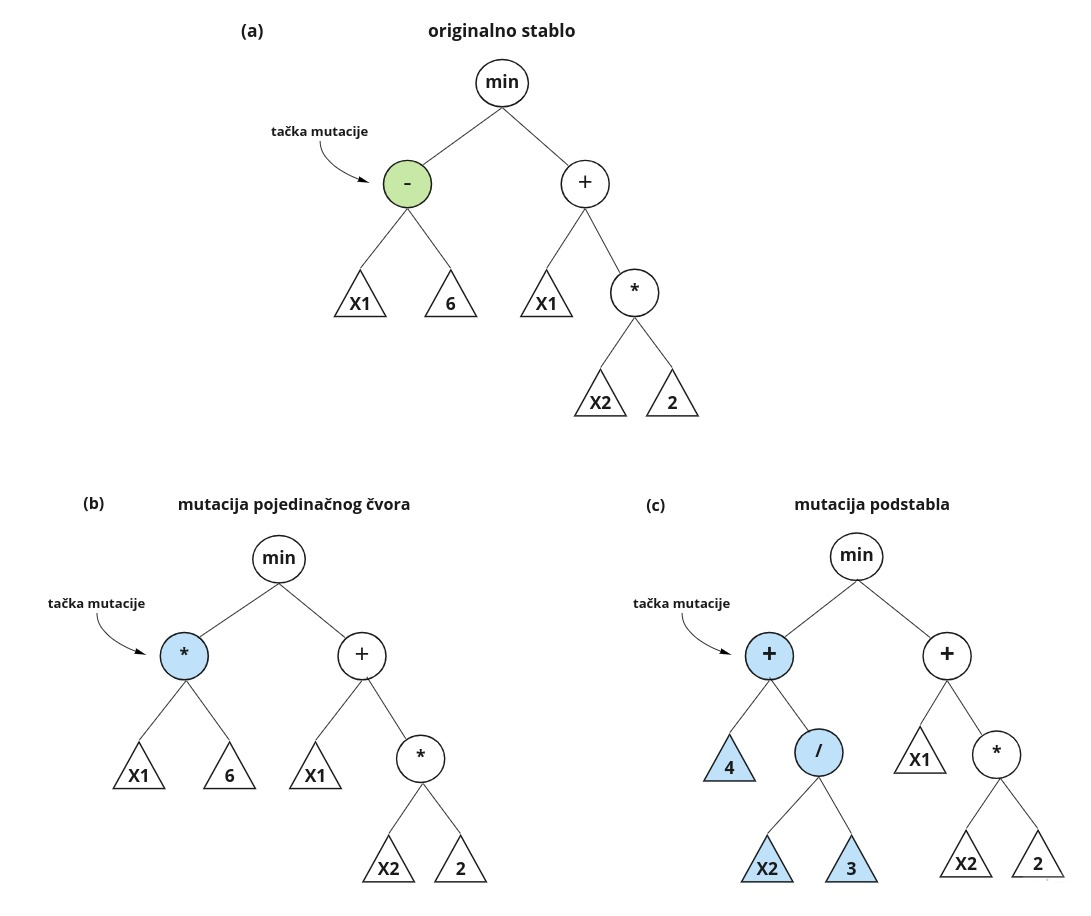
\includegraphics[width=0.65\textwidth]{images/mutation4.jpg}
\end{center}
\label{fig:mutation}
\end{figure}

\end{enumerate}
\end{frame}

\begin{frame}{Zaustavljanje}
Evolutivni proces stvaranja novih generacija se ponavlja sve dok nije zadovoljen neki uslov zaustavljanja:
\begin{enumerate}
    \item Pronađeno je rešenje koje zadovoljava unapred zadati kriterijum.
    \item Dostignut je zadati broj generacija.
    \item Dostignut je definisani vremenski kriterijum zaustavljanja.
    \item Funkcija prilagođenosti je izračunata zadati broj puta.
\end{enumerate}
Ovde su korišćeni uslovi 1, 2 i 3, pri čemu se u uslovu 1. smatra da je pronađeno zadovoljavajuće rešenje ako mu je "adjusted" funkcija prilagođenosti veća od 0.9. 
\end{frame}

\subsection{Metoda promenljivih okolina}
\begin{frame}{Metoda promenljivih okolina (VNS, eng. \textit{Variable Neighbourhood Search}) \cite{vnp}}
\scriptsize
\begin{itemize}
    \item S-metaheuristika (Single-solution-based metaheuristika) - zasnovana na lokalnoj pretrazi i unapred̄ivanju jednog rešenj.
    \item VNS metoda je zasnovana na 3 činjenice:
    \begin{enumerate}
    \scriptsize
        \item Lokalni optimum u odnosu na jednu okolinu ne mora da predstavlja lokalni optimum u odnosu na drugu.
        \item Globalni optimum je lokalni optimum u odnosu na sve moguće okoline.
        \item Za mnoge probleme lokalni optimumi u odnosu na različite okoline su relativno blizu.
    \end{enumerate}
    \item Činjenica 3. ukazuje na to da lokalni optimum često daje neke informacije o globalnom. Zato se okoline lokalnog optimuma istražuju u potrazi za boljim rešenjem u nadi da će pretraga dovesti do globalnog optimuma.
    \item Osnovnu varijantu metode promenljivih okolina (Basic VNS, eng. \textit{Basic Variable Neighbourhood Search}) čine lokalna pretraga i stohastička procedura razmrdavanja (eng. \textit{shaking}).
    \item Cilj razmrdavanja je da spreči da se pretraga zaglavi u nekom lokalnom optimumu.
\end{itemize}
\end{frame}

\begin{frame}{Metoda promenljivih okolina}
\begin{enumerate}
  \item Inicijalizacija: Izbor skupa okolina $N_k, k = 1, ..., k_{max}$; Konstruisanje početnog rešenja x; Izbor kriterijuma zaustavljanja.
  \item Ponavljanje narednih koraka sve dok se ne ispuni kriterijum zaustavljanja:
  \begin{enumerate}
    \item Postaviti k = 1
    \item Ponavljati naredne korake sve dok je $k \leq k_{max}$
        \begin{enumerate}
        \item \textit{Razmrdavanje} - Generisanje slučajnog rešenja $x'$ iz okoline $N_k(x)$ ;
        \item \textit{Lokalna pretraga} - Primeniti neku metodu lokalne pretrage sa početnim rešenjem $x'$. Rezultat pretrage označiti sa $x''$;
        \item \textit{Prihvatanje rešenja i promena okoline} - Ako je tako dobijeno rešenje $x''$ bolje od  $x$, postaviti $x$ = $x''$ i  $k = 1$; Inače, postaviti $k = k + 1$;
      \end{enumerate}
  \end{enumerate}
\end{enumerate}
\end{frame}


\begin{frame}{Tipovi okolina}
\begin{enumerate}
    \item  $N(T)$ - struktura susedstva koje se koristi tokom lokalne pretrage. Članovi ove vrste susedstva se formiraju elementarnim transformacijama stabla.
    \item $N_1(T)$ - struktura susedstva čiji se članovi dobijaju zamenom samo jednog čvora početnog stabla $T$. Odgovara operatoru mutacije pojedinačnog čvora kod GP.
    \item $N_2(T)$ predstavlja operator zamene (eng. \textit{Swap operator}). Odgovara operatoru mutacije celog podstabla kod GP.
\end{enumerate}
Okoline $N_1(T)$ i $N_2(T)$ se koriste u proceduri razmrdavanja.
\end{frame}

\begin{frame}{Razmrdavanje}
\begin{itemize}
    \small
    \item Dobija se $k$-ti sused stabla $T$, primenom istog poteza $k$ puta.
    \item Prvo se nasumičnobira okolina $N_1(T)$ ili $N_2(T)$, a zatim se taj operator primenjuje $k$ puta nad datim stablom.
\end{itemize}
\begin{figure}[!ht]
\begin{center}
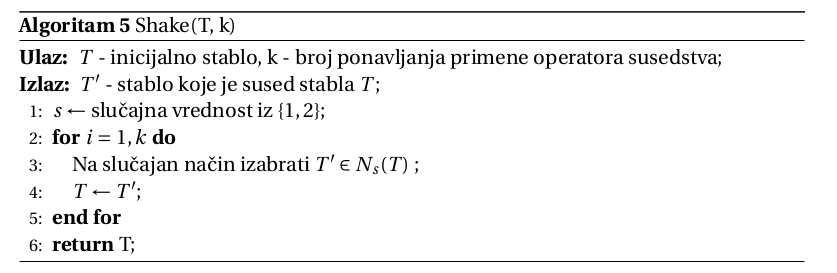
\includegraphics[width=0.9\textwidth]{images/shake_alg.png}
\end{center}
\label{fig:mutation}
\end{figure}
\end{frame}

\begin{frame}{Elementarne transformacije stabla (ETT) i lokalna pretraga}
\begin{itemize}
\small
    \item Susedi koji se razmatraju tokom lokalne pretrage se generišu elementarnim transformacijama trenutno najboljeg rešenja.
    \item Elementarne transformacije stabla (ETT, eng. \textit{Elementary Tree Transformation}) se definišu na sledeći način. Neka je $G(V, E)$ neusmereni graf sa skupom čvorova $V$ i skupom grana $E$ i neka je $T(V, A)$ neko razapinjuće stablo grafa $G$. ETT transformiše stablo $T$ u stablo $T'$ (u oznaci $T' = ETT(T)$) sledećim koracima:
    \begin{enumerate}
        \item U stablo $T$ dodati granu $a$, takvu da $a \in E \setminus A$.
        \item Detektovati formirani ciklus i ukloniti bilo koju granu (osim one koja je dodata u prethodnom koraku) iz njega kako bi se dobio podgraf $T'$, koji takođe predstavlja razapinjuće stablo grafa $G$.
    \end{enumerate}
\end{itemize}
\end{frame}

\begin{frame}{Elementarne transformacije stabla (ETT) i lokalna pretraga}
\begin{figure}[!ht]
\begin{center}
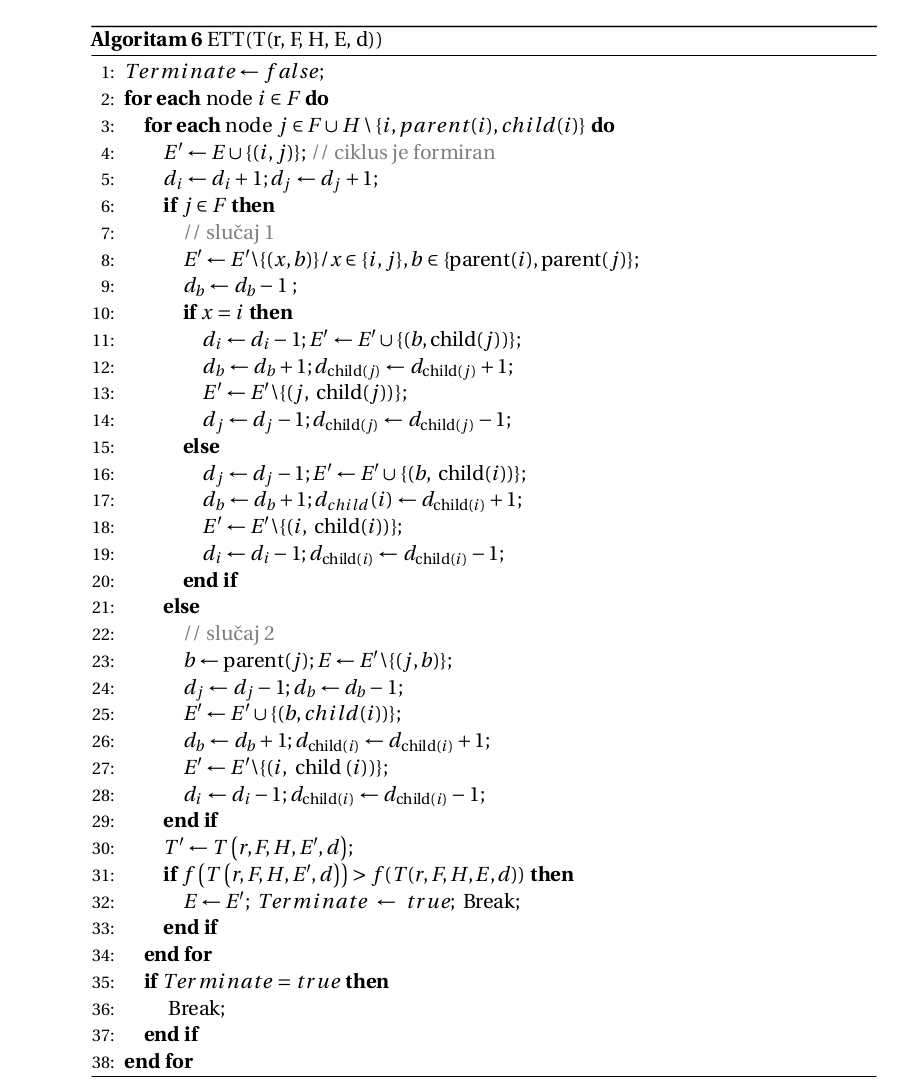
\includegraphics[width=0.52\textwidth]{images/ett_alg.png}
\end{center}
\end{figure}

\end{frame}

\begin{frame}{Elementarne transformacije stabla (ETT) i lokalna pretraga}
\scriptsize
Naredbe algoritma se se mogu grupisati u četiri grupe (dve vrste dodavanja grane i dve vrste uklanjanja grane):
\begin{enumerate}
    \item \textit{Dodavanje grane (tip I)} (linije 4,5). Grana $(i,j)$ se dodaje u trenutno stablo $T$, pri čemu ni $i$ ni $j$ ne smeju biti koren stabla. Dodatno, ili $i$ ili $j$ mora da bude funkcija. Nakon primene ovog koraka se formira ciklus u trenutnom stablu.
    \item \textit{Uklanjanje grane (tip I)} (linije 8,9,23,24). Ovde postoje dva slučaja. Ako su i $i$ i $j$ funkcije (slučaj 1 u algoritmu), onda se može ukloniti neka od grana $(i, parent(i))$, $(j, parent(j))$ kako bi se uklonio ciklus. Ako je jedan od čvorova terminal, npr. neka to bude $j$, onda se uklanja grana $(j, parent(j))$ (slučaj 2 u algoritmu).
    \item \textit{Dodavanje grane (tip II)} (linije 11,12,16,17,25,26). Ako je obrisana grana $(i, parent(i))$, onda se dodaje grana $(parent(i), child(j))$. Ako je obrisana grana $(j, parent(j))$, onda se dodaje grana $(parent(j), child(i))$. 
    \item \textit{Uklanjanje grane (tip II)} (linije 13,14,18,19,27,28). Ove grane se uklanjaju kako bi stepen čvorova ostao zadovoljavajući. 
\end{enumerate}
\end{frame}


\begin{frame}{Elementarne transformacije stabla (ETT) i lokalna pretraga}
\begin{itemize}
    \item Pomoću ETT je implementirana lokalna pretraga koja koristi strategiju \textit{prvog poboljšanja}.
    \item Kada se naiđe na prvo stablo koje daje bolje rezultate na datom skupu podataka, ono se vraća kao trenutno najbolje rešenje iz čijeg susedstva će se dalje nastaviti pretraga.
    \item Kao funkcija na osnovu koje se poredi kvaliet stabala, uzet je koeficijent determinacije $R^{2}$. 
\end{itemize}
\end{frame}

\begin{frame}{Algoritam osnovne metode promenljivih okolina}
\begin{figure}[!ht]
\begin{center}
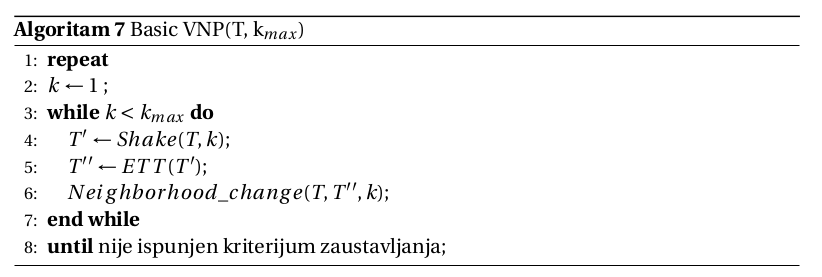
\includegraphics[width=0.9\textwidth]{images/vnp_alg.png}
\end{center}
\end{figure}
\begin{itemize}
    \item Kriterijum zaustavljanja biti pronalazak tačnog rešenja, maksimalan dozvoljeni broj iteracija ili maksimalno vreme izvršavanja.
\end{itemize}
\end{frame}

\section{Eksperimentalni rezultati}

\begin{frame}{Podaci}
Sve metode su testirane pomoću tri vrste skupova podataka:
\begin{enumerate}
\small
    \item Skup podataka generisan na osnovu funkcija koje se često razmatraju u literaturi. Za svaku funkciju je generisano 100 instanci na osnovu slučajno odabranih vrednosti nezavisnih promenljiih. Funkcije i intervali vrednosti iz kojeg su birane tačke su:
    
    $ F_1 = x^3 + x^2 + x, \quad x \in [-1, 1] $

    $ F_2 = x^4 + x^3 + x^2 + x, \quad x \in [-1, 1] $
    
    $ F_3 = x^5 + x^4 + x^3 + x^2 + x, \quad x \in [-1, 1] $
    
    $ F_4 = x^6 + x^5 + x^4 + x^3 + x^2 + x, \quad x \in [-1, 1] $
    
    $ F_5 = sin(x^2)cos(x) - 1, \quad x \in [-1, 1] $
    
    $ F_6 = sin(x) + sin(x + x^2), \quad x \in [-1, 1] $
    
    $ F_7 = log(x + 1) + log(x^2 + 1), \quad x \in [0, 2] $
    
    $ F_8 = sin(x_0) + sin(x_1^2), \quad x_0, x_1 \in [-1, 1] $
    
    $ F_9 = 2sin(x_0)cos(x_1), \quad x_0, x_1 \in [-1, 1] $
\end{enumerate}
\end{frame}

\begin{frame}{Podaci}
\begin{enumerate}
\setcounter{enumi}{1}
    \item Skup podataka generisan na osnovu jednostavnijih funkcija radi upoređivanja metaheurističkih metoda sa metodom grube sile.
    
    $F_{01} = x_0 x_1 + x_1$

    $F_{02} = x_1 + x_1^2 + x_0$
    
    $F_{03} = x_0 x_1 + cos(x_0)$
    
    $F_{04} = x_0 - x_1 x_1$
    
    $F_{05} = x_0 - x_1 x_1 + x_1$
\end{enumerate}
\end{frame}

\begin{frame}{Podaci}
\begin{enumerate}
\setcounter{enumi}{2}
    \item Jedan od javno dostupnih skupova podataka za regresiju - $"$Yacht Hydrodynamics$"$ skup. Kod njega je cilj predvideti vrednost rezidualnog otpora jahte na osnovu njenih karakteristika. Skup sadrži 308 instanci koje su određene pomoću 6 nezavisnih i jedne ciljne promenljive. Sve vrednosti su realnog tipa.
\end{enumerate}
\end{frame}

\begin{frame}{Evaluacija algoritma grube sile i poređenje sa metaheurističkim metodama}
\begin{itemize}
    \item Algoritam grube sile je uspešno mogao da dođe do optimalnog rešenja za primere $F_{01}, ..., F_{05}$ i $F_{1}$ i $F_{2}$.
    \item U ostalim primerima je, nakon više sati izvršavanja, dolazilo do nedostatka memorijskih resursa, bez pronalaska dovoljno dobrog rešenja.
    \item Svi metaheuristički pristupi su, uspešno pronašli optimalno rešenje za primere $F_{01}, ..., F_{05}$.
\end{itemize}
\end{frame}

\begin{frame}{Evaluacija algoritma grube sile i poređenje sa metaheurističkim metodama}
\small
\begin{table}
\caption{Vreme izvršavanja (izraženo u sekundama) svih metoda na poblemima manjih dimenzija}
\label{tbl:bruteForceResults}
\begin{center}
\begin{tabular}{ |c|c|c|c|c| } 
\hline
\thead{} & \thead{Algoritam \\ grube sile} & \thead{GP} & \thead{GP sa SSC} & \thead{VNP} \\
\hline
$\boldsymbol F_{\boldsymbol 0 \boldsymbol 1}$ & 1 & 12 & 19 & 4 \\ 
\hline
$\boldsymbol F_{\boldsymbol 0 \boldsymbol 2}$ & <1 & 7 & 13 & 6 \\ 
\hline
$\boldsymbol F_{\boldsymbol 0 \boldsymbol 3}$ & <1 & 6 & 12 & 6 \\ 
\hline
$\boldsymbol F_{\boldsymbol 0 \boldsymbol 4}$ & <1 & 12 & 18 & 5 \\ 
\hline
$\boldsymbol F_{\boldsymbol 0 \boldsymbol 5}$ & <1 & 7 & 18 & 6 \\ 
\hline
$\boldsymbol F_{\boldsymbol 1}$ & <1 & 15 & 24 & 7 \\ 
\hline
$\boldsymbol F_{\boldsymbol 2}$ & 22 & 13 & 26 & 8 \\ 
\hline
\end{tabular}
\end{center}
\end{table}

\end{frame}


\begin{frame}{Evaluacija i poređenje metaheurističkih metoda}
\begin{itemize}
    \item Svaki skup podataka je podeljen na trening (70\%) i test (30\%) deo.
    \item Svaka metoda je evaluirana tako što je pokrenuta po 30 puta nad svim skupovima podataka.
    \item Prilikom svakog od tih nezavisnih pokretanja dobijen je izraz koji u tom izvršavanju najbolje odgovara datom skupu podataka. 
    \item Za taj izraz je zatim izračunat koeficijent determinacije $R^2$ na trening i test skupu i provereno je da li i simbolički odgovara ciljnom izrazu.
    \item Pri svakom pokretanju mereno je i vreme koje je bilo potrebno za pronalazak najboljeg rešenja.
\end{itemize}
\end{frame}

%--------------------------

\begin{frame}{Evaluacija i poređenje metaheurističkih metoda}
\scriptsize
\begin{table}[ht]
\caption{Vrednosti parametara genetskog programiranja} 
\label{tbl:gpParameters}
\centering
\begin{tabular}{l l} % centered columns (4 columns)
\hline 
Parametar & Vrednost \\ [0.5ex] 
\hline 
Veličina populacije & 500  \\ 
Maksimalan broj generacija & 50  \\
Broj jedinki za reprodukciju & 300  \\
Veličina turnira & 3 \\
Verovatnoća mutacie pojedinačnog čvora & 0.2  \\
Verovatnoća mutacije celog podstabla & 0.2  \\ 
Minimalna dubina stabla & 2 \\
Maksimalna dubina stabla u fazi inicijalizacije & 6 \\
Maksimalna veličina stabla & 16 \\
Vrsta funkcije prilagođenosti & adjusted \\ 
Skup funkcija &  +, -, *, /, pow, sin, cos, log \\ [1ex] % [1ex] adds vertical space
\hline 
\end{tabular}
\end{table}
\end{frame}


\begin{frame}{Evaluacija i poređenje metaheurističkih metoda}
\scriptsize
\begin{table}[ht]
\caption{Vrednosti parametara genetskog programiranja za "Yacht Hydrodynamics" skup podataka} 
\label{tbl:gpParametersYacht}
\centering
\begin{tabular}{l l} % centered columns (4 columns)
\hline 
Parametar & Vrednost \\ [0.5ex] 
\hline 
Veličina populacije & 2000  \\ 
Maksimalan broj geneacija & 100  \\
Broj jedinki za reprodukciju & 1200  \\
Veličina turnira & 10 \\
Verovatnoća mutacie pojedinačnog čvora & 0.2  \\
Verovatnoća mutacije celog podstabla & 0.2  \\ 
Minimalna dubina stabla & 2 \\
Maksimalna dubina stabla u fazi inicijalizacije & 12 \\
Maksimalna veličina stabla & 64 \\
Vrsta funkcije prilagođenosti & adjusted \\ 
Skup funkcija &  +, -, *, /, pow, sin, cos, log \\ [1ex] % [1ex] adds vertical space
\hline 
\end{tabular}
\end{table}
\end{frame}

\begin{frame}{Evaluacija i poređenje metaheurističkih metoda}
\scriptsize
\begin{table}[H]
\caption{Vrednosti parametara metode promenljivih okolina} 
\label{tbl:vnpParameters}
\centering
\begin{tabular}{l l} % centered columns (4 columns)
\hline 
Parametar & Vrednost \\ [0.5ex] 
\hline 
$k_{max}$ & 4  \\ 
Minimalna dubina stabla & 2 \\
Maksimalna dubina stabla u fazi inicijalizacije & 4 \\
Maksimalna dubina stabla kreiranog u fazi prerage  & 6 \\
Maksimalan broj iteracija & 1000 \\ 
Skup funkcija &  +, -, *, /, pow, sin, cos, log \\ [1ex] % [1ex] adds vertical space
\hline 
\end{tabular}
\end{table}

Kod "Yacht" skupa je za $k_{max}$ uzeta vrednost 6, a broj iteracija je povećan na 2000.

\end{frame}

%------------------------------------------

\begin{frame}{Evaluacija i poređenje metaheurističkih metoda}
\scriptsize

\newcolumntype{?}{!{\vrule width 1pt}}
\begin{table}
\caption{Prosečne vrednosti određenih karakteristika u 30 nezavisnih pokretanja}
\begin{center}
\begin{tabular}{ |c?|c|c|c?|c|c|c?| } 
\hline
& \multicolumn{3}{|c?|}{\thead{Prosečna \bm{$R^2$} vrednost \\ na  trening skupu}} & \multicolumn{3}{|c?|}{\thead{Prosečna \bm{$R^2$} vrednost \\ na test skupu}} \\
\hline
& \textbf{GP} & \textbf{GP sa SSC} & \textbf{VNP} & \textbf{GP} & \textbf{GP sa SSC} & \textbf{VNP} \\
\hline
$\boldsymbol F_{\boldsymbol 0 \boldsymbol 1}$ & 0.879 & 0.831 & \textbf{0.949} & 0.898 & 0.861 & \textbf{0.945} \\
\hline
$\boldsymbol F_{\boldsymbol 0 \boldsymbol 2}$ & 0.765 & 0.802 & \textbf{0.848} & 0.791 & 0.818 & \textbf{0.897} \\
\hline
$\boldsymbol F_{\boldsymbol 0 \boldsymbol 3}$ & 0.745 & 0.733 & \textbf{0.863} & 0.810 & 0.820 & \textbf{0.926} \\
\hline
$\boldsymbol F_{\boldsymbol 0 \boldsymbol 4}$ & 0.733 & 0.740 & \textbf{0.914} & 0.820 & 0.775 & \textbf{0.922} \\
\hline
$\boldsymbol F_{\boldsymbol 0 \boldsymbol 5}$ & 0.795 & 0.771 & \textbf{0.846} & 0.797 & 0.765 & \textbf{0.813} \\
\hline
\end{tabular}
\end{center}
\end{table}

\end{frame}

\begin{frame}{Evaluacija i poređenje metaheurističkih metoda}
\scriptsize

\newcolumntype{?}{!{\vrule width 1pt}}
\begin{table}
\caption{Prosečne vrednosti određenih karakteristika u 30 nezavisnih pokretanja}
\begin{center}
\begin{tabular}{ |c?|c|c|c?|c|c|c?| } 
\hline
& \multicolumn{3}{|c?|}{\thead{Broj pokretanja u kojima je \\ pronađeno rešenje \\ simbolički ekvivalentno \\ ciljnom rešenju}} & \multicolumn{3}{|c|}{\thead{Prosečno vreme \\ izvršavanja (s)}}  \\
\hline
& \textbf{GP} & \textbf{GP sa SSC} & \textbf{VNP} & \textbf{GP} & \textbf{GP sa SSC} & \textbf{VNP} \\
\hline
$\boldsymbol F_{\boldsymbol 0 \boldsymbol 1}$ & 7 & 3 & \textbf{13} & 12 & 19 & \textbf{4} \\
\hline
$\boldsymbol F_{\boldsymbol 0 \boldsymbol 2}$ & 1 & 3 & \textbf{11} & 7 & 13 & \textbf{6} \\
\hline
$\boldsymbol F_{\boldsymbol 0 \boldsymbol 3}$ & 5 & 5 & \textbf{14} & 6 & 12 & \textbf{5} \\
\hline
$\boldsymbol F_{\boldsymbol 0 \boldsymbol 4}$ & 2 & 1 & \textbf{9} & 12 & 18 & \textbf{5} \\
\hline
$\boldsymbol F_{\boldsymbol 0 \boldsymbol 5}$ & 3 & 1 & \textbf{9} & \textbf{7} & 18 & \textbf{7} \\
\hline
\end{tabular}
\end{center}
\end{table}

\end{frame}


%  ////////////////////////////////




\begin{frame}{Evaluacija i poređenje metaheurističkih metoda}
\scriptsize
\newcolumntype{?}{!{\vrule width 1pt}}
\begin{table}
\caption{Prosečne vrednosti određenih karakteristika u 30 nezavisnih pokretanja}
\label{tbl:meanVals2}
\begin{center}
\begin{tabular}{ |c?|c|c|c?|c|c|c?| } 
\hline
& \multicolumn{3}{|c?|}{\thead{Prosečna \bm{$R^2$} vrednost \\ na  trening skupu}} & \multicolumn{3}{|c?|}{\thead{Prosečna \bm{$R^2$} vrednost \\ na test skupu}}  \\
\hline
& \textbf{GP} & \textbf{GP sa SSC} & \textbf{VNP} & \textbf{GP} & \textbf{GP sa SSC} & \textbf{VNP} \\
\hline
$\boldsymbol F_{\boldsymbol 1}$ & \textbf{0.914} & 0.861 & 0.907 & \textbf{0.907} & 0.827 & 0.872 \\
\hline
$\boldsymbol F_{\boldsymbol 2}$ & \textbf{0.827} & 0.799 & 0.771 & \textbf{0.824} & 0.798 & 0.770 \\
\hline
$\boldsymbol F_{\boldsymbol 3}$ & \textbf{0.851} & 0.851 & 0.797 & 0.695 & -1.428 & \textbf{0.752} \\
\hline
$\boldsymbol F_{\boldsymbol 4}$ & 0.746 & 0.691 & \textbf{0.809} & \textbf{0.796} & 0.743 & 0.778 \\
\hline
$\boldsymbol F_{\boldsymbol 5}$ & 0.643 & 0.606 & \textbf{0.894} & 0.607 & 0.589 & \textbf{0.887} \\
\hline
$\boldsymbol F_{\boldsymbol 6}$ & 0.928 & 0.917 & \textbf{0.945} & 0.883 & 0.881 & \textbf{0.930} \\
\hline
$\boldsymbol F_{\boldsymbol 7}$ & 0.960 & 0.968 & \textbf{0.994} & 0.950 & 0.959 & \textbf{0.993} \\
\hline
$\boldsymbol F_{\boldsymbol 8}$ & 0.857 & 0.837 & \textbf{0.968} & 0.716 & 0.657 & \textbf{0.936} \\
\hline
$\boldsymbol F_{\boldsymbol 9}$ & 0.950 & 0.940 & \textbf{0.963} & 0.955 & 0.938 & \textbf{0.971} \\
\hline
\end{tabular}
\end{center}
\end{table}
\end{frame}



\begin{frame}{Evaluacija i poređenje metaheurističkih metoda}
\scriptsize
\newcolumntype{?}{!{\vrule width 1pt}}
\begin{table}
\caption{Prosečne vrednosti određenih karakteristika u 30 nezavisnih pokretanja}
\label{tbl:meanVals2}
\begin{center}
\begin{tabular}{ |c?|c|c|c?|c|c|c?| } 
\hline
& \multicolumn{3}{|c?|}{\thead{Broj pokretanja u kojima je \\ pronađeno rešenje \\ simbolički ekvivalentno \\ ciljnom rešenju}} & \multicolumn{3}{|c|}{\thead{Prosečno vreme \\ izvršavanja (s)}}  \\
\hline
& \textbf{GP} & \textbf{GP sa SSC} & \textbf{VNP} & \textbf{GP} & \textbf{GP sa SSC} & \textbf{VNP}  \\
\hline
$\boldsymbol F_{\boldsymbol 1}$ & 0 & 0 & \textbf{13} & 15 & 24 & \textbf{7} \\
\hline
$\boldsymbol F_{\boldsymbol 2}$ & 0 & 0 & \textbf{9} & 13 & 26 & \textbf{9} \\
\hline
$\boldsymbol F_{\boldsymbol 3}$ & 0 & 0 & \textbf{2} & 20 & 23 & \textbf{10} \\
\hline
$\boldsymbol F_{\boldsymbol 4}$ & 0 & 0 & \textbf{2} & 14 & 27 & \textbf{12} \\
\hline
$\boldsymbol F_{\boldsymbol 5}$ & 0 & 0 & 0 & \textbf{14} & 24 & \textbf{14} \\
\hline
$\boldsymbol F_{\boldsymbol 6}$ & 0 & 0 & \textbf{1} & 13 & 27 & \textbf{12} \\
\hline
$\boldsymbol F_{\boldsymbol 7}$ & 0 & 0 & 0 & 18 & 51 & \textbf{13} \\
\hline
$\boldsymbol F_{\boldsymbol 8}$ & 0 & 0 & \textbf{3} & 13 & 35 & \textbf{7} \\
\hline
$\boldsymbol F_{\boldsymbol 9}$ & 1 & 1 & \textbf{2} & 12 & 28 & \textbf{8} \\
\hline
\end{tabular}
\end{center}
\end{table}
\end{frame}



%///////////////////////////////////////



\begin{frame}{Evaluacija i poređenje metaheurističkih metoda}
\scriptsize
\begin{table}
\caption{Prosečne vrednosti određenih karakteristika u 30 nezavisnih pokretanja za "Yacht Hydrodynamics" skup podataka}
\label{tbl:meanVals3}
\begin{center}
\begin{tabular}{ |c|c|c|c|c| } 
\hline
\thead{Metoda} & \thead{Prosečna \bm{$R^2$} \\ vrednost na \\ trening skupu} & \thead{Prosečna \bm{$R^2$} \\ vrednost na \\ test skupu} &  \thead{Prosečno vreme \\ izvršavanja (s)} \\
\hline
\multirow{1}{*}{GP} 
& 0.238 & 0.264 & 183 \\
\hline
\multirow{1}{*}{GP sa SSC}
& 0.213 & 0.233 & 247  \\
\hline
\multirow{1}{*}{VNP} 
& \textbf{0.477} & \textbf{0.457} & \textbf{30} \\
\hline
\end{tabular}
\end{center}
\end{table}
\end{frame}


%-------------------------------------------------------------------------



\begin{frame}{Evaluacija i poređenje metaheurističkih metoda}
\tiny
\newcolumntype{?}{!{\vrule width 1pt}}
\begin{table}
\caption{Informacije o izrazu koji daje maksimalnu $R^2$ vrednost na test skupu od svih izraza dobijenih pri 30 nezavisnih pokretanja}
\label{tbl:maxVals1}
\begin{center}
\begin{tabular}{ |c?|c|c|c?|c|c|c?| } 
\hline
& \multicolumn{3}{|c?|}{\thead{Maksimalna \bm{$R^2$} vrednost \\ na  test skupu}} & \multicolumn{3}{|c?|}{\thead{Izraz koji ima maksimalnu \\ \bm{$R^2$} vrednost na test skupu}} \\
\hline
& \textbf{GP} & \textbf{GP sa SSC} & \textbf{VNP} & \textbf{GP} & \textbf{GP sa SSC} & \textbf{VNP} \\
\hline
$\boldsymbol F_{\boldsymbol 0 \boldsymbol 1}$ & 1.0 & 1.0 & 1.0 & $x_1(x_0$ + $1)$ & $x_1(x_0$ + $1)$ & $x_1(x_0$ + $1)$ \\
\hline
$\boldsymbol F_{\boldsymbol 0 \boldsymbol 2}$ & 1.0 & 1.0 & 1.0 & $x_0$ + $x_1^2$ + $x_1$ & $x_0$ + $x_1^2$ + $x_1$ & $x_0$ + $x_1^2$ + $x_1$  \\
\hline
$\boldsymbol F_{\boldsymbol 0 \boldsymbol 3}$ & 1.0 & 1.0 & 1.0 & $x_0 x_1$ + $cos(x_0)$ & $x_0 x_1$ + $cos(x_0)$ & $x_0 x_1$ + $cos(x_0)$ \\
\hline
$\boldsymbol F_{\boldsymbol 0 \boldsymbol 4}$ & 1.0 & 1.0 & 1.0 & $x_0 - x_1^2$ & $x_0 - x_1^2$ & $x_0 - x_1^2$  \\
\hline
$\boldsymbol F_{\boldsymbol 0 \boldsymbol 5}$ & 1.0 & 1.0 & 1.0 & $x_0 - x_1^2$ + $x_1$ & $x_0 - x_1^2$ + $x_1$ & $x_0 - x_1^2$ + $x_1$ \\
\hline
\end{tabular}
\end{center}
\end{table}
\end{frame}



\begin{frame}{Evaluacija i poređenje metaheurističkih metoda}
\scriptsize
\newcolumntype{?}{!{\vrule width 1pt}}
\begin{table}
\caption{Informacije o izrazu koji daje maksimalnu $R^2$ vrednost na test skupu od svih izraza dobijenih pri 30 nezavisnih pokretanja}
\label{tbl:maxVals1}
\begin{center}
\begin{tabular}{ |c?|c|c|c?| } 
\hline
& \multicolumn{3}{|c|}{\thead{Simbolička \\ ekvivalencija sa \\ ciljnim izrazom}} \\
\hline
& \textbf{GP} & \textbf{GP sa SSC} & \textbf{VNP} \\
\hline
$\boldsymbol F_{\boldsymbol 0 \boldsymbol 1}$ & Da & Da & Da \\
\hline
$\boldsymbol F_{\boldsymbol 0 \boldsymbol 2}$ & Da & Da & Da \\
\hline
$\boldsymbol F_{\boldsymbol 0 \boldsymbol 3}$ & Da & Da & Da \\
\hline
$\boldsymbol F_{\boldsymbol 0 \boldsymbol 4}$ & Da & Da & Da \\
\hline
$\boldsymbol F_{\boldsymbol 0 \boldsymbol 5}$ & Da & Da & Da \\
\hline
\end{tabular}
\end{center}
\end{table}
\end{frame}

%///////////////////////////////////////
% -------------------


\begin{frame}{Evaluacija i poređenje metaheurističkih metoda}
\tiny
\newcolumntype{?}{!{\vrule width 1pt}}
\renewcommand{\arraystretch}{1.0}
\begin{table}
\caption{Informacije o izrazu koji daje maksimalnu $R^2$ vrednost na test skupu od svih izraza dobijenih pri 30 nezavisnih pokretanja}
\label{tbl:maxVals2}
\begin{center}
\begin{tabular}{ |c?|c|c|c?|c|c|c| } 
\hline
& \multicolumn{3}{|c?|}{\thead{Maksimalna \\ \bm{$R^2$} vrednost \\ na  test skupu}} & \multicolumn{3}{|c|}{\thead{Simbolička \\ ekvivalencija sa \\ ciljnim izrazom}} \\
\hline
& \textbf{GP} & \textbf{\thead{GP \\ sa SSC}} & \textbf{VNP} & \textbf{GP} & \textbf{\thead{GP \\ sa SSC}} & \textbf{VNP} \\
\hline
$\boldsymbol F_{\boldsymbol 1}$ & 0.992 & 0.985 & \textbf{1.0} & Ne & Ne & \textbf{Da} \\
\hline
$\boldsymbol F_{\boldsymbol 2}$ & 0.994 & 0.981 & \textbf{1.0} & Ne & Ne & \textbf{Da} \\
\hline
$\boldsymbol F_{\boldsymbol 3}$ & 0.981 & 0.995 & \textbf{1.0} & Ne & Ne & \textbf{Da} \\
\hline
$\boldsymbol F_{\boldsymbol 4}$ & 0.986 & 0.960 & \textbf{1.0} & Ne & Ne & \textbf{Da}  \\
\hline
$\boldsymbol F_{\boldsymbol 5}$ & 0.943 & 0.964 & \textbf{0.999} & Ne & Ne & Ne \\
\hline
$\boldsymbol F_{\boldsymbol 6}$ & 0.971 & 0.987 & \textbf{1.0} & Ne & Ne & \textbf{Da} \\
\hline
$\boldsymbol F_{\boldsymbol 7}$ & 0.997 & 0.998 & \textbf{0.999} & Ne & Ne & Ne \\
\hline
$\boldsymbol F_{\boldsymbol 8}$ & 0.999 & 0.994 & \textbf{1.0} & Ne & Ne & \textbf{Da} \\
\hline
$\boldsymbol F_{\boldsymbol 9}$ & \textbf{1.0} & \textbf{1.0} & \textbf{1.0} & \textbf{Da} & \textbf{Da} & \textbf{Da} \\
\hline
\end{tabular}
\end{center}
\end{table}

\end{frame}

\begin{frame}{Evaluacija i poređenje metaheurističkih metoda}
\scriptsize
\begin{table}
\def\arraystretch{1.5}
\caption{Informacije o izrazu koji daje maksimalnu $R^2$ vrednost na test skupu od svih izraza dobijenih pri 30 nezavisnih pokretanja za "Yacht Hydrodynamics" skup podataka}
\label{tbl:maxVals3}
\begin{center}
\setlength{\extrarowheight}{4pt}
\begin{tabular}{ |c|c|c|c|c| } 
\hline
\thead{Metoda} & \thead{Maksimalna \bm{$R^2$} \\ vrednost na \\ test skupu} & \thead{Izraz koji ima \\ maksimalnu \bm{$R^2$} \\ vrednost na \\ test skupu } \\
\hline
{GP} & 0.929 & $1.906^{(3.963 x_5)}$  \\
\hline
{GP sa SSC} & 0.792 & $ \frac{0.822}{0.052^{x_5}} $ \\
\hline
{VNP} 
& \textbf{0.956} & $ 0.000196^{\frac{x_1 - x_2 x_5}{x_2}  * \frac{x_5}{x_1 - 2 x_5^2} } $ \\
\hline
\end{tabular}
\end{center}
\end{table}
\end{frame}


\section{Literatura}
\begin{frame}[allowframebreaks]
        \frametitle{Literatura}
        \bibliographystyle{abbrv}
        \bibliography{literature.bib}
\end{frame}


\setbeamertemplate{footline}{\hspace*{.5cm}\scriptsize{\hspace*{50pt} \hfill\hspace*{.5cm} \setbeamercolor{black}}\\
\vspace{9pt}}

\setbeamertemplate{headline}{\hspace*{.5cm}\scriptsize{\hspace*{50pt} \hfill\hspace*{.5cm} \setbeamercolor{black}}\\
\vspace{1pt}}

% \setbeamercolor{mysection in head/foot}{bg= black,fg=black}
\end{document}